\chapter{Introduction}
This paper discusses two security measurements, namely Link Layer Security (LLSEC) and Datagram TLS (DTLS), within Contiki OS.

\section{Related Work}
\cite{802154Sec} discusses some security concerns in 802.15.4.  LLSEC\cite{LLSEC} is the implementation of 802.15.4 security in Contiki.

tinydtls\cite{tinydtls} is the implementation of DTLS we used in DTLS related experiments.

\section{Experiment Setup}
All experiments are done within the Cooja simulator.

The setup is as described in \Cref{fig: Setup}.

\begin{figure}
\centering{
	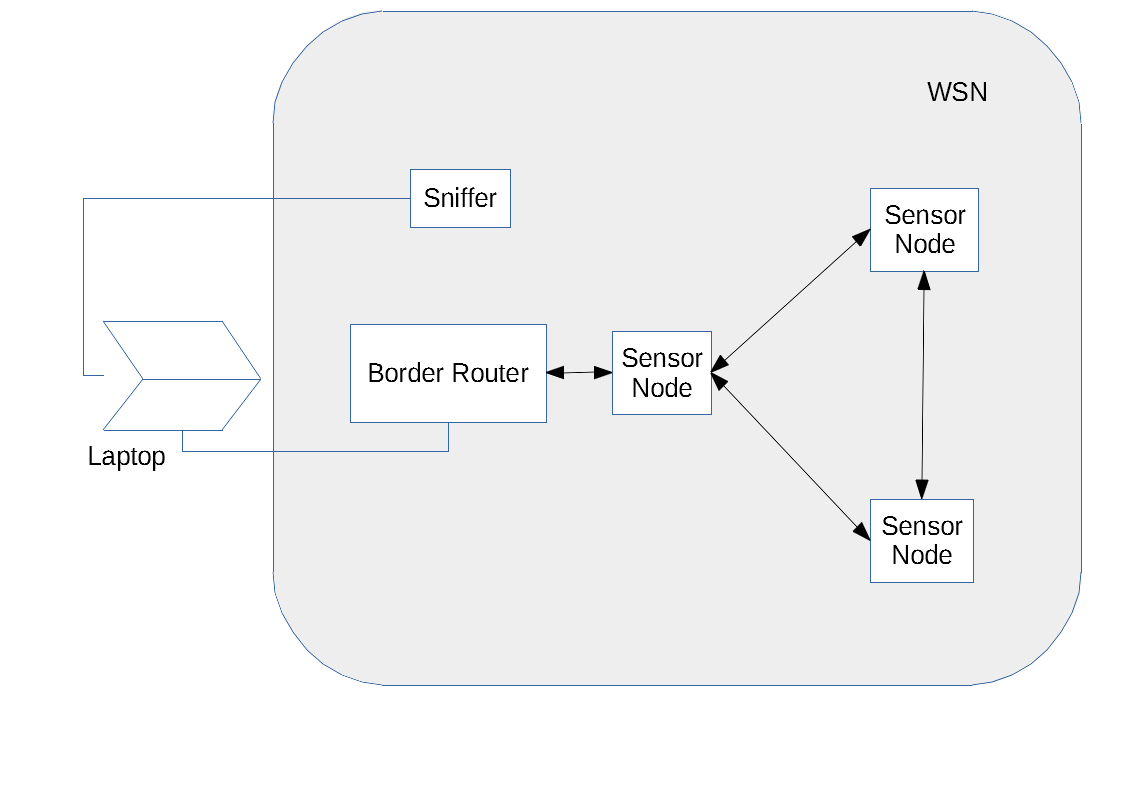
\includegraphics[width=1\textwidth]{fig/setup.png}
}
\caption{Experiment setup} \label{fig: Setup}
\end{figure}

\begin{itemize}
\item{\bf Adversary} is the malicious party that tries to recover information from the encrypted traffic.
\item{\bf Border Router}, or BR, is a device that connects the adversary to the sensor network. However, this is only allowed when LLSEC is disabled. 
\item{\bf Sniffer} is a device that passively captures all traffics in the sensor network. 
\item{\bf Target} and {\bf Nodes} are sensors deployed in the sensor network. They communicates to each other through encrypted channels.
\end{itemize}